\chapter{Dari Bahan Baku sampai Daur Ulang}\label{ch:g5:raw-materials-and-recycling}

Sebuah kaleng minuman kosong dijatuhkan ke tempat sampah \omterm{def:g5:raw-materials-and-recycling:recycling}{daur ulang}.
Sebuah truk membawanya ke pusat pemilahan, sebuah mesin memampatkannya
menjadi balok bersama ribuan kaleng lain, sebuah tanur melelehkan
balok-balok itu, dan beberapa minggu kemudian logam itu kembali ke rak
toko sebagai kaleng baru. Dari mana logam itu berasal pada mulanya, dan
mengapa kaleng bekas layak dilelehkan alih-alih membuat logam baru?

\begin{recall}
Benda adalah sesuatu yang dapat kita lihat dan sentuh; bahannya adalah
apa yang membentuknya --- kayu, logam, kaca, plastik, kertas, kain, batu
(\cref{ch:g1:materials-around-us}). Pada \omterm{def:g5:irreversible-changes:chemical-change}{perubahan kimia}, zat-zat baru
muncul dan tidak ada jalan kembali yang sederhana
(\cref{ch:g5:irreversible-changes}).
\end{recall}

\section{Bahan alami dan bahan buatan}

\begin{definition}[Bahan alami dan bahan buatan]\label{def:g5:raw-materials-and-recycling:natural-material}
Sebuah \emph{bahan alami}\index{bahan alami} dipakai hampir seperti
ketika ditemukan di alam, hanya dipotong atau dibentuk: kayu, batu,
katun, wol, kulit. Sebuah \emph{bahan buatan}\index{bahan buatan}
dibuat manusia dari zat-zat yang ditemukan di alam, dengan mengubahnya,
sering kali dengan panas dan \omterm{def:g5:irreversible-changes:chemical-change}{perubahan kimia}: kaca, baja, aluminium,
plastik, kertas, beton.
\end{definition}

\begin{example}[Dua meja]\label{ex:g5:raw-materials-and-recycling:tables}
Meja dari papan kayu jati terbuat dari \omterm{def:g5:raw-materials-and-recycling:natural-material}{bahan alami}: kayunya hanya
digergaji, diketam, dan dilem. Meja dengan daun meja kaca dan kaki baja
terbuat dari \omterm{def:g5:raw-materials-and-recycling:natural-material}{bahan buatan}: baik kaca maupun baja tidak ditemukan dalam
bentuk itu di alam.
\end{example}

\section{Bahan baku}

\begin{definition}[Bahan baku dan bijih]\label{def:g5:raw-materials-and-recycling:raw-material}
Yang disebut \emph{bahan baku}\index{bahan baku} adalah zat yang
diambil dari alam untuk membuat bahan dan benda: pohon, pasir, batuan,
minyak bumi, kapas, wol. Batuan yang darinya sebuah logam diambil
disebut \emph{bijih}\index{bijih}.
\end{definition}

\begin{example}[Asal bahan-bahan]\label{ex:g5:raw-materials-and-recycling:from}
\begin{itemize}
  \item kayu dan kertas berasal dari pohon;
  \item kaca berasal dari pasir yang dipanaskan sangat kuat bersama soda
        dan batu kapur;
  \item besi dan baja berasal dari \omterm{def:g5:raw-materials-and-recycling:raw-material}{bijih} besi, batuan yang kemerahan;
  \item aluminium berasal dari bauksit, \omterm{def:g5:raw-materials-and-recycling:raw-material}{bijih} yang lain;
  \item kebanyakan plastik berasal dari minyak bumi, yang dipompa dari
        dalam tanah;
  \item katun berasal dari tanaman kapas, wol dari domba.
\end{itemize}
\end{example}

\begin{omfigure}
\begin{minipage}[b]{0.48\linewidth}\centering
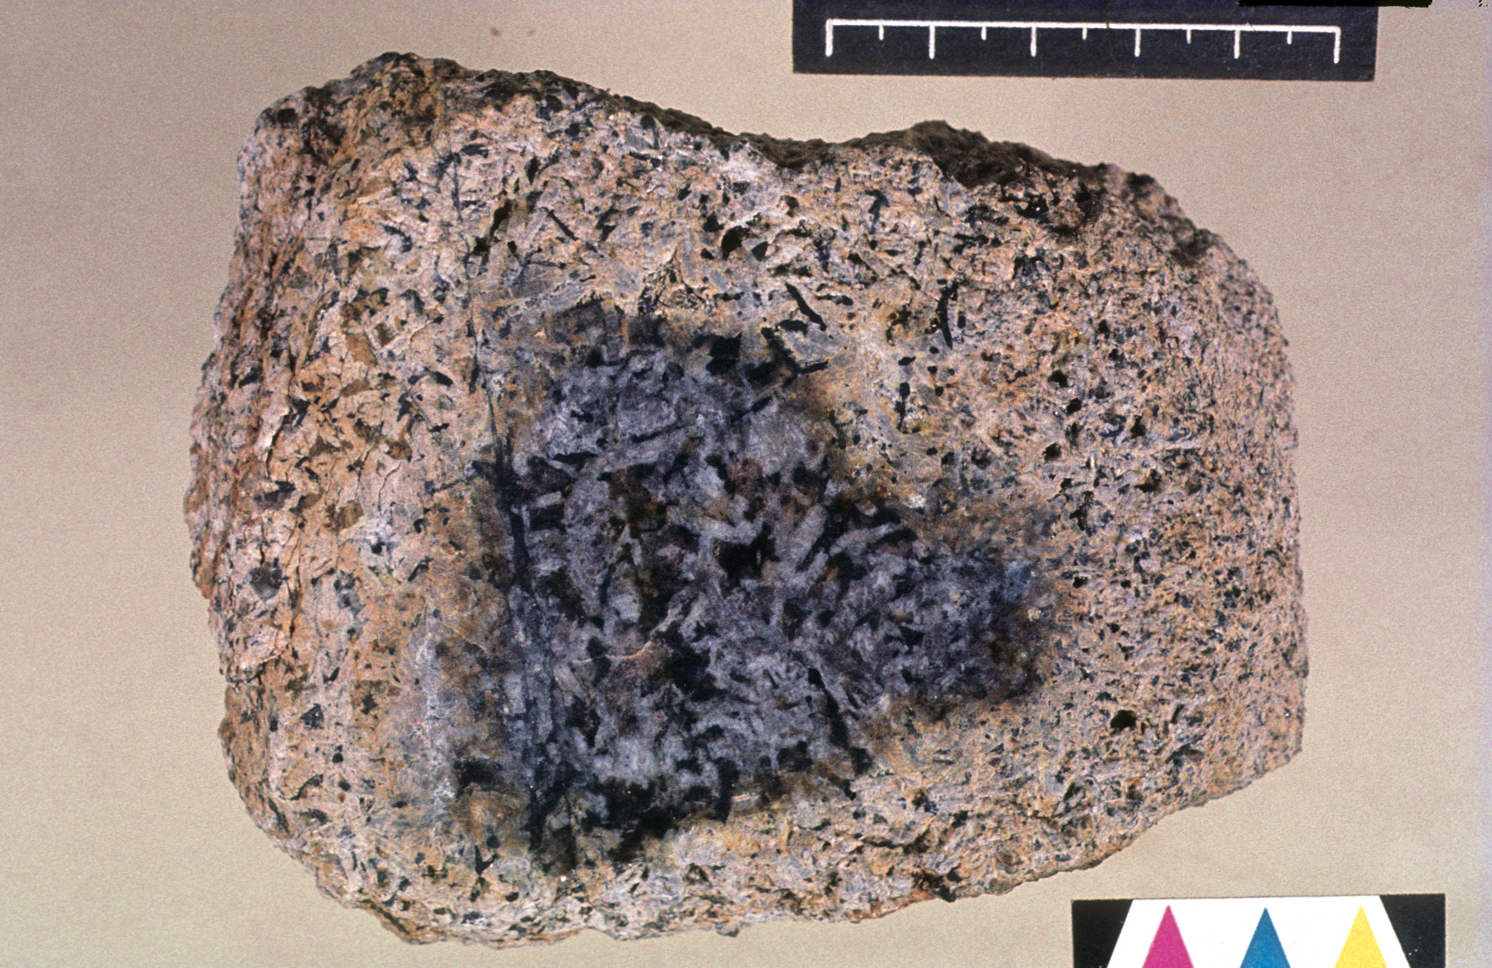
\includegraphics[width=\linewidth,height=4.6cm,keepaspectratio]{images/book1/bauxite.jpg}

{\small Bauksit, \omterm{def:g5:raw-materials-and-recycling:raw-material}{bijih} aluminium, mengelilingi inti batuan yang belum
lapuk. Foto: Werner Schellmann, CC\ BY-SA\ 2.5.}
\end{minipage}\hfill
\begin{minipage}[b]{0.48\linewidth}\centering
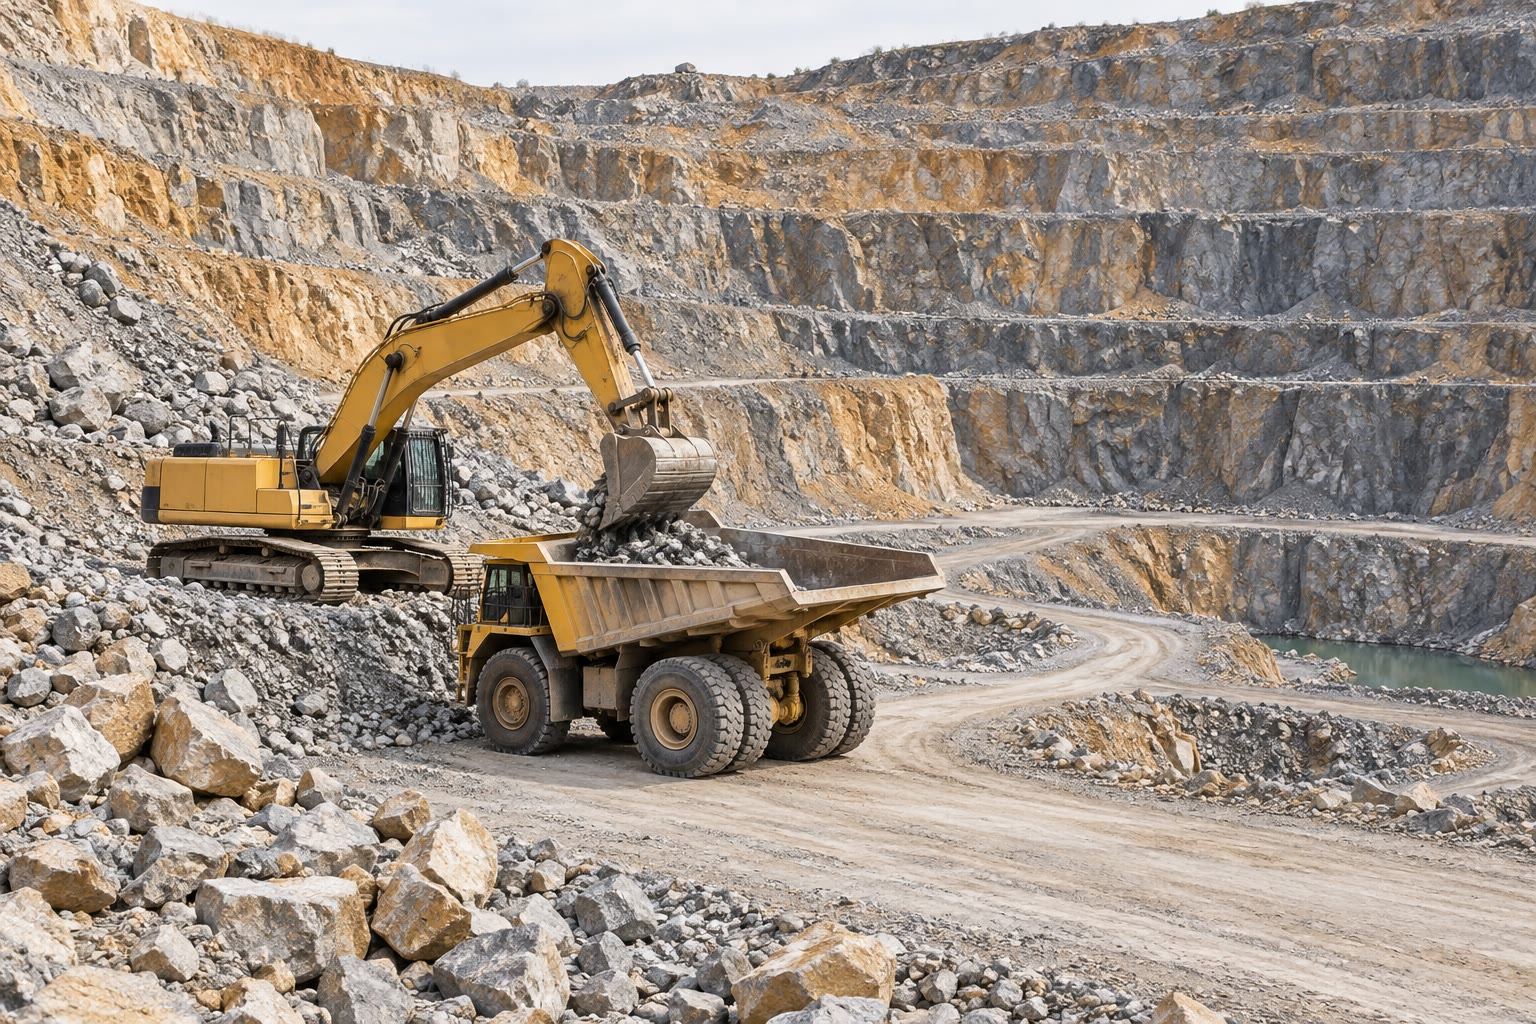
\includegraphics[width=\linewidth,height=4.6cm,keepaspectratio]{images/book1/ai/g5-quarry.jpg}

{\small Tambang batu: batuan digali untuk dipakai sebagai \omterm{def:g5:raw-materials-and-recycling:raw-material}{bahan baku}.}
\end{minipage}
\end{omfigure}

\begin{omfigure}
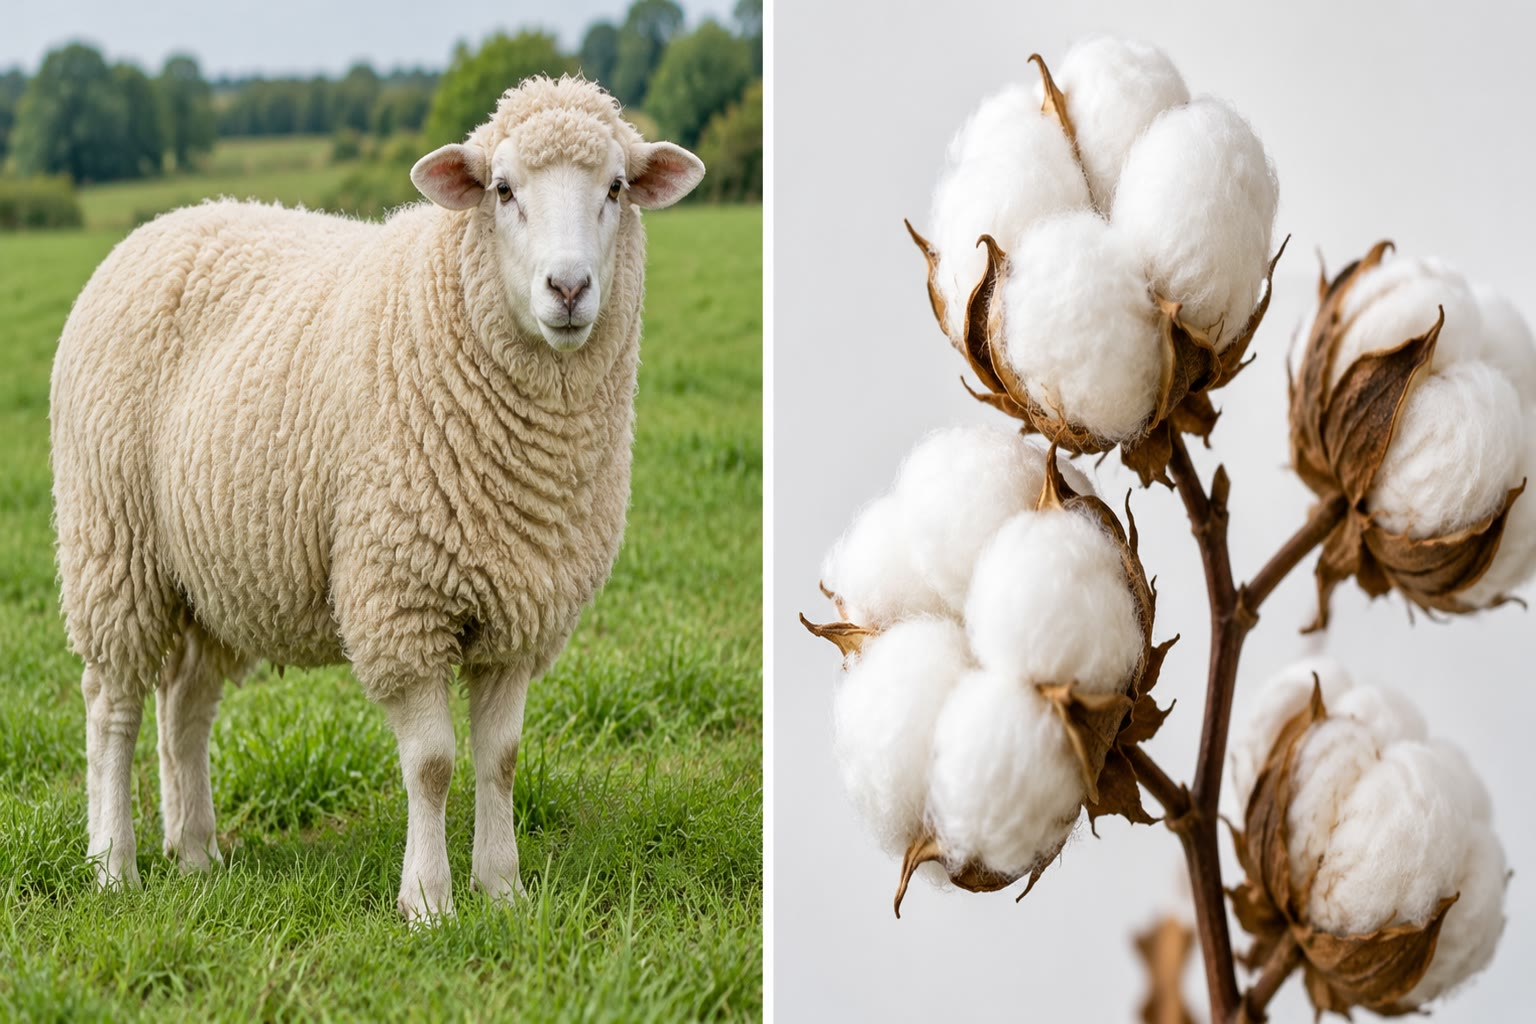
\includegraphics[width=0.6\linewidth]{images/book1/ai/g5-sheep-cotton.jpg}

{\small \omterm{def:g5:raw-materials-and-recycling:raw-material}{Bahan baku} alami dari makhluk hidup: wol dari domba, kapas dari
tanaman kapas.}
\end{omfigure}

\section{Dari bahan baku menjadi benda}

\begin{proposition}[Membuat bahan mengubah bahan bakunya]\label{prop:g5:raw-materials-and-recycling:change}
Mengubah \omterm{def:g5:raw-materials-and-recycling:raw-material}{bahan baku} menjadi \omterm{def:g5:raw-materials-and-recycling:natural-material}{bahan buatan} memerlukan energi --- paling
sering panas sebuah tanur --- dan biasanya \omterm{def:g5:irreversible-changes:chemical-change}{perubahan kimia}: pasir
menjadi kaca, \omterm{def:g5:raw-materials-and-recycling:raw-material}{bijih} menjadi logam, minyak menjadi plastik. Perubahan
ini tidak dapat dibalik begitu saja: kaca tidak kembali menjadi pasir.
\end{proposition}

\begin{example}[Riwayat sebuah botol kaca]\label{ex:g5:raw-materials-and-recycling:bottle}
Pasir, soda, dan batu kapur yang dihancurkan dipanaskan bersama di
dalam tanur sampai melebur menjadi kaca. Kaca yang panas ditiup menjadi
bentuk botol. Botol itu diisi, dijual, dan dikosongkan. Kalau dimasukkan
ke wadah pengumpul botol, botol itu dihancurkan menjadi kepingan kecil,
dilelehkan lagi, dan ditiup menjadi botol baru: kacanya dipakai lagi dan
lagi.
\end{example}

\begin{omfigure}
\begin{tikzpicture}[font=\small,
    box/.style={draw=omDef, fill=omDef!6, rounded corners=2pt, align=center,
      minimum height=0.95cm, text width=2.4cm}]
  \node[box] (r) at (0,2.6) {bahan baku\\ (pasir, bijih, minyak)};
  \node[box] (m) at (4.0,2.6) {pembuatan\\ bahan};
  \node[box] (o) at (8.0,2.6) {benda,\\ dipakai};
  \node[box] (w) at (8.0,0) {sampah};
  \node[box, draw=omProp, fill=omProp!8] (s) at (4.0,0) {pemilahan dan\\ daur ulang};
  \draw[->, thick, omDef] (r) -- (m);
  \draw[->, thick, omDef] (m) -- (o);
  \draw[->, thick, omDef] (o) -- (w);
  \draw[->, thick, omProp] (w) -- (s);
  \draw[->, thick, omProp] (s) -- (m) node[midway, left, align=right, text=black]
    {dipakai lagi\\ pengganti\\ bahan baku baru};
  \draw[->, thick, black!45, dashed] (w.east) -- ++(1.4,0) node[right, align=left,
    text=black] {dibuang:\\ ke TPA};
\end{tikzpicture}

{\small Riwayat sebuah bahan. Lingkaran jingga adalah \omterm{def:g5:raw-materials-and-recycling:recycling}{daur ulang}: bahan
dari benda lama menggantikan \omterm{def:g5:raw-materials-and-recycling:raw-material}{bahan baku} baru.}
\end{omfigure}

\section{Pemilahan dan daur ulang}

\begin{definition}[Daur ulang]\label{def:g5:raw-materials-and-recycling:recycling}
Yang disebut \emph{daur ulang}\index{daur ulang} adalah mengumpulkan
benda-benda bekas dan mengolah bahannya agar dapat dibuat menjadi
benda baru, alih-alih dibuang.
\end{definition}

\begin{proposition}[Mengapa mendaur ulang]\label{prop:g5:raw-materials-and-recycling:why}
% ledger: al:energy-primary, al:energy-recycled (8.3 / 186 = about 1/22)
\omterm{def:g5:raw-materials-and-recycling:recycling}{Daur ulang} menghemat \omterm{def:g5:raw-materials-and-recycling:raw-material}{bahan baku}, yang tidak perlu digali dari dalam
tanah, dan sering kali menghemat energi. Membuat aluminium dari kaleng
bekas hanya memerlukan sekitar seperdua puluh energi yang diperlukan
untuk membuatnya dari bauksit. \omterm{def:g5:raw-materials-and-recycling:recycling}{Daur ulang} juga berarti lebih sedikit
sampah di tempat pembuangan akhir.
\end{proposition}

\begin{method}[Memilah sampah untuk didaur ulang]\label{met:g5:raw-materials-and-recycling:sort}
\omterm{def:g5:raw-materials-and-recycling:recycling}{Daur ulang} dimulai dengan pemilahan, di mana pun sampah dibuang:
\begin{enumerate}
  \item botol dan stoples kaca di satu tempat sampah;
  \item kaleng logam, kertas dan karton, serta botol plastik di tempat
        sampah yang disediakan kota untuk masing-masing (warna tempat
        sampah berbeda dari satu tempat ke tempat lain);
  \item yang tidak dapat didaur ulang bersama sampah lainnya.
\end{enumerate}
Setiap bahan didaur ulang dengan caranya sendiri, jadi sebuah tempat
sampah hanya boleh berisi bahan yang memang diperuntukkan baginya.
\end{method}

\begin{omfigure}
\begin{tikzpicture}[font=\small]
  \foreach \k/\t/\bc in {0/kaca/green!50!black, 1/{kaleng logam}/gray,
                        2/{kertas dan karton}/omDef, 3/{botol plastik}/orange!80!black} {
    \begin{scope}[xshift=\k*3.4cm]
      \fill[\bc!18, draw=\bc, line width=0.8pt] (-1,0) -- (1,0) -- (1.15,2.0)
        -- (-1.15,2.0) -- cycle;
      \fill[\bc!45, draw=\bc] (-1.25,2.0) rectangle (1.25,2.3);
      \node[anchor=north, align=center] at (0,-0.15) {\t};
    \end{scope}
  }
  % glass: a bottle
  \fill[green!40!black!60] (-0.2,0.3) rectangle (0.2,1.2);
  \fill[green!40!black!60] (-0.07,1.2) rectangle (0.07,1.6);
  % metal: a can
  \begin{scope}[xshift=3.4cm]
    \fill[black!25, draw=black!55] (-0.3,0.3) rectangle (0.3,1.3);
  \end{scope}
  % paper: a box and a sheet
  \begin{scope}[xshift=6.8cm]
    \fill[brown!25, draw=brown!60] (-0.6,0.3) rectangle (0.1,1.0);
    \fill[white, draw=black!40] (0.2,0.3) rectangle (0.65,1.3);
  \end{scope}
  % plastic: a bottle
  \begin{scope}[xshift=10.2cm]
    \fill[cyan!20, draw=cyan!50!black] (-0.25,0.3) rectangle (0.25,1.3);
    \fill[cyan!20, draw=cyan!50!black] (-0.1,1.3) rectangle (0.1,1.6);
  \end{scope}
\end{tikzpicture}

{\small Empat tempat sampah pemilahan, satu untuk setiap bahan. (Warna
tempat sampah yang sebenarnya berbeda dari kota ke kota.)}
\end{omfigure}

\begin{omfigure}
\begin{minipage}[t]{0.48\linewidth}\centering
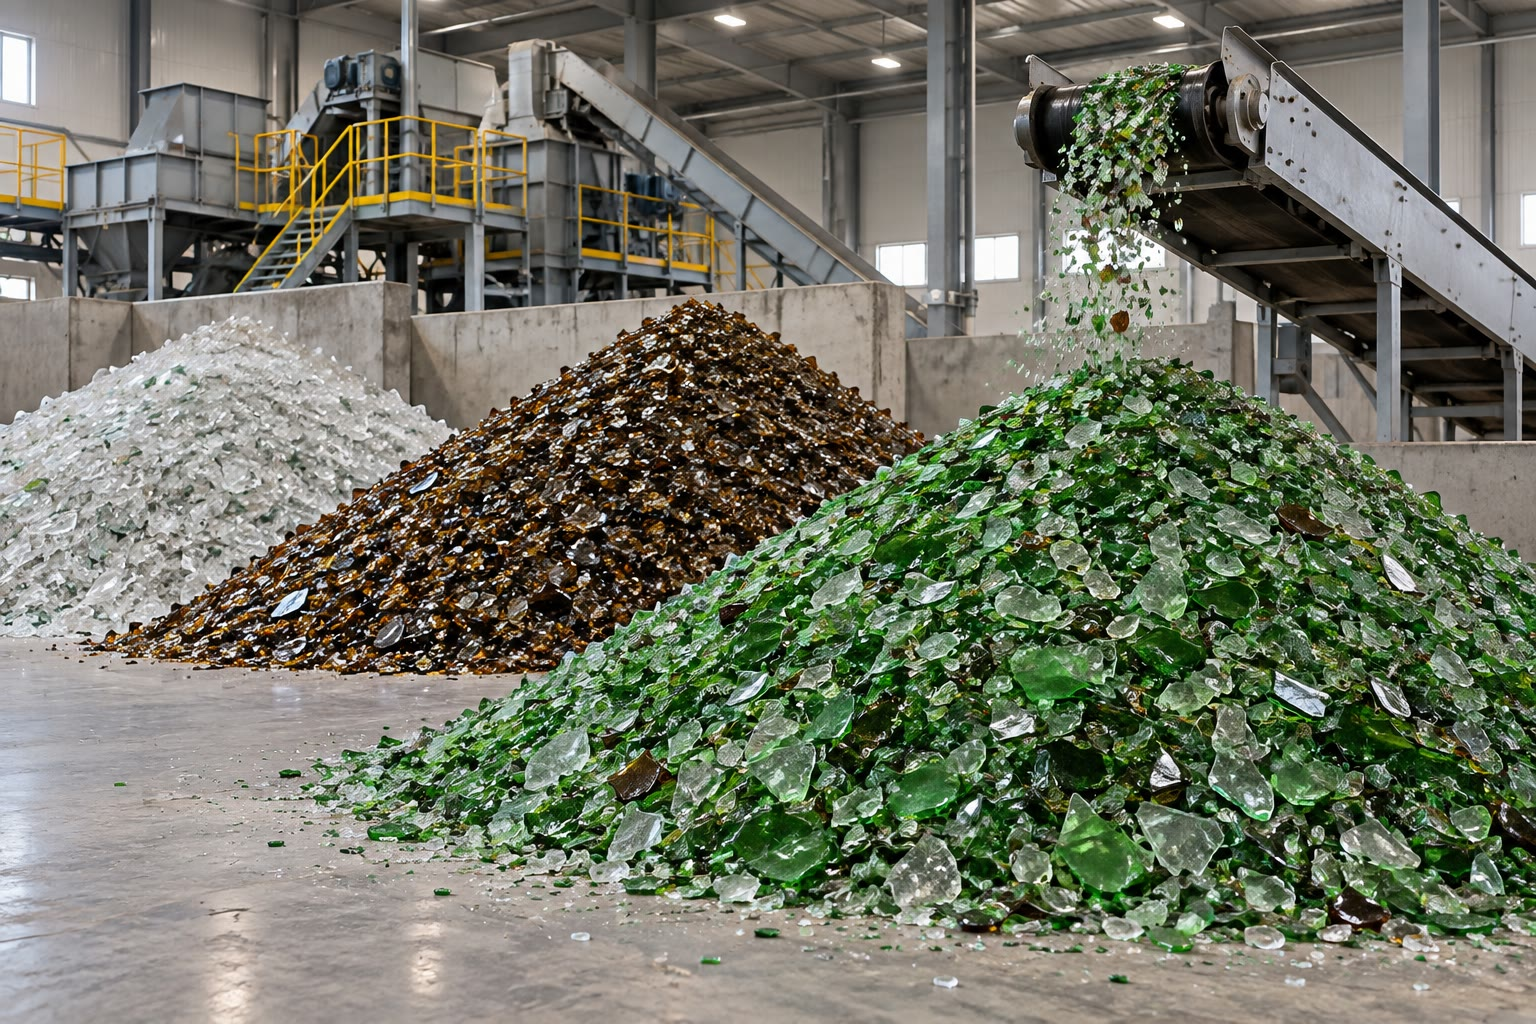
\includegraphics[width=\linewidth,height=4.6cm,keepaspectratio]{images/book1/ai/g5-glass-cullet.jpg}

{\small Kaca yang dihancurkan di pabrik \omterm{def:g5:raw-materials-and-recycling:recycling}{daur ulang}, siap dilelehkan.}
\end{minipage}\hfill
\begin{minipage}[t]{0.48\linewidth}\centering
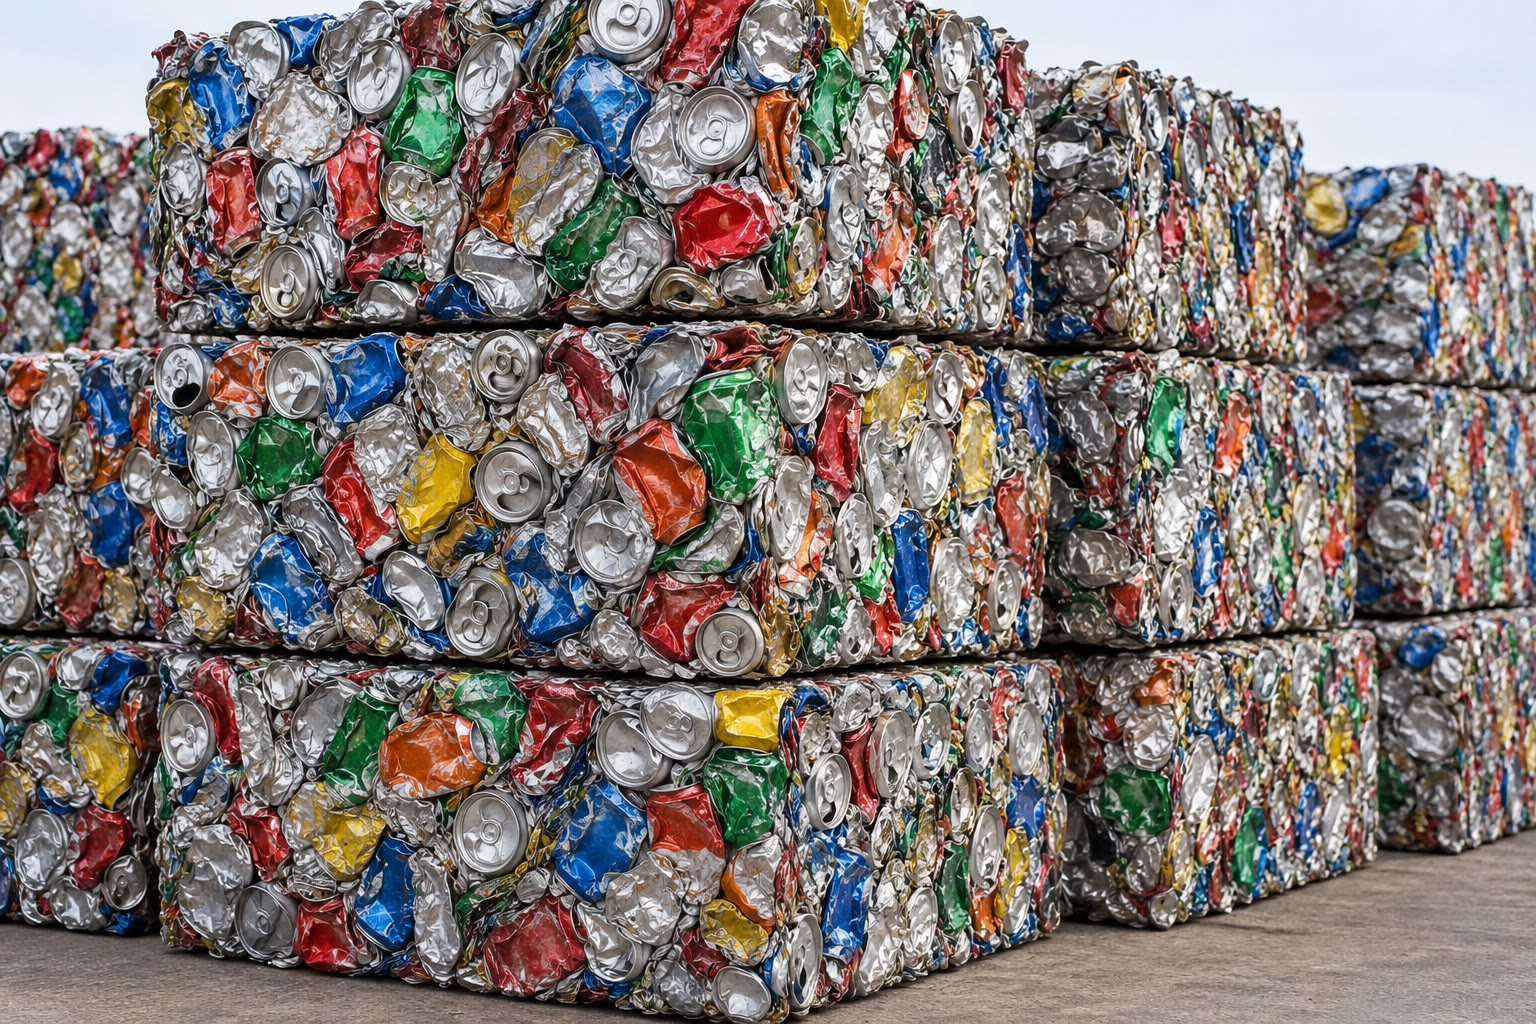
\includegraphics[width=\linewidth,height=4.6cm,keepaspectratio]{images/book1/ai/g5-can-bales.jpg}

{\small Bongkahan kaleng aluminium yang dipampatkan.}
\end{minipage}
\end{omfigure}

\section{Sampah dan sumber daya}

\begin{definition}[Sumber daya]\label{def:g5:raw-materials-and-recycling:resource}
Yang disebut \emph{sumber daya}\index{sumber daya} adalah apa saja
yang diambil dari alam dan dipakai manusia: air, kayu, \omterm{def:g5:raw-materials-and-recycling:raw-material}{bijih}, minyak,
pasir. Sebuah \emph{sumber daya
terbarukan}\index{sumber daya terbarukan} tumbuh kembali atau datang
kembali dengan sendirinya dalam rentang hidup manusia, seperti kayu
dari hutan yang ditanami kembali atau wol dari domba. \omterm{def:g5:raw-materials-and-recycling:raw-material}{Bijih} dan minyak
bumi tidak terbarukan: sekali digali dan dipakai, keduanya habis.
\end{definition}

\begin{proposition}[Kurangi, gunakan kembali, daur ulang]\label{prop:g5:raw-materials-and-recycling:three}
Agar \omterm{def:g5:raw-materials-and-recycling:resource}{sumber daya} bertahan lama, orang dapat melakukan, dengan urutan
ini:
\begin{enumerate}
  \item \textbf{kurangi}: memakai lebih sedikit benda, misalnya lebih
        sedikit pembungkus;
  \item \textbf{gunakan kembali}: memakai benda yang sama lagi, seperti
        stoples kaca yang diisi ulang atau tas yang dibawa kembali ke
        toko;
  \item \textbf{\omterm{def:g5:raw-materials-and-recycling:recycling}{daur ulang}}: mengubah bahannya menjadi benda baru.
\end{enumerate}
\omterm{def:g5:raw-materials-and-recycling:recycling}{Daur ulang} ditempatkan terakhir karena masih memerlukan energi dan
mesin; sampah terbaik adalah sampah yang tidak pernah dibuat.
\end{proposition}

\section{Latihan}

\begin{exercise}[$\star$]\label{exo:g5:raw-materials-and-recycling:1}
Alami atau buatan? Kayu, kaca, wol, baja, plastik, batu.
\end{exercise}

\begin{exercise}[$\star$]\label{exo:g5:raw-materials-and-recycling:2}
Sebutkan \omterm{def:g5:raw-materials-and-recycling:raw-material}{bahan baku} dari: selembar kertas, stoples kaca, kaus katun,
botol plastik.
\end{exercise}

\begin{exercise}[$\star$]\label{exo:g5:raw-materials-and-recycling:3}
Apa itu \omterm{def:g5:raw-materials-and-recycling:raw-material}{bijih}? Sebutkan \omterm{def:g5:raw-materials-and-recycling:raw-material}{bijih} aluminium.
\end{exercise}

\begin{exercise}[$\star$]\label{exo:g5:raw-materials-and-recycling:4}
Di tempat sampah mana kamu memasukkan: stoples selai kosong, koran,
kaleng minuman, botol air minum plastik?
\end{exercise}

\begin{exercise}[$\star$]\label{exo:g5:raw-materials-and-recycling:5}
Lihatlah gambar riwayat sebuah bahan. Apa yang digantikan oleh
lingkaran jingga?
\end{exercise}

\begin{exercise}[$\star$]\label{exo:g5:raw-materials-and-recycling:6}
Terbarukan atau tidak: kayu, minyak bumi, wol, \omterm{def:g5:raw-materials-and-recycling:raw-material}{bijih} besi, kapas?
\end{exercise}

\begin{exercise}[$\star$]\label{exo:g5:raw-materials-and-recycling:7}
Mengapa kaca tidak dapat diubah kembali menjadi pasir dengan
mendinginkannya?
\end{exercise}

\begin{exercise}[$\star$]\label{exo:g5:raw-materials-and-recycling:8}
Berikan satu cara mengurangi, satu cara menggunakan kembali, dan satu
cara mendaur ulang.
\end{exercise}

\begin{exercise}[$\star$]\label{exo:g5:raw-materials-and-recycling:9}
Mengapa tempat sampah kaca hanya boleh berisi kaca?
\end{exercise}

\begin{exercise}[$\star\star$]\label{exo:g5:raw-materials-and-recycling:10}
Membuat aluminium dari kaleng bekas memerlukan sekitar seperdua puluh
energi yang diperlukan untuk membuatnya dari bauksit. Sebuah pabrik
memakai 20 satuan energi untuk membuat sejumlah aluminium dari
bauksit. Kira-kira berapa satuan yang akan dipakainya untuk membuat
jumlah yang sama dari kaleng bekas?
\end{exercise}

\begin{exercise}[$\star\star$]\label{exo:g5:raw-materials-and-recycling:11}
Mengapa ``kurangi'' ditempatkan sebelum ``\omterm{def:g5:raw-materials-and-recycling:recycling}{daur ulang}''?
\end{exercise}
